% %\documentclass[12pt]{article}
% \documentclass[12pt,onecolumn]{revtex4-1}
% %\documentstyle[aps,multicol,eincludegraphics]{revtex}
% %\documentclass[twocolumn]{revtex4}
% \usepackage{graphicx}
% %\usepackage{scicite}
% % \usepackage{epstopdf}
% \usepackage{amsmath}
% %\usepackage{times}
% 
% \topmargin 0.0cm
% \oddsidemargin 0.2cm
% \textwidth 16cm 
% \textheight 21cm
% \footskip 1.0cm
% 
% 
% 
% 
% \begin{document}
% 
% 
% \noindent
% {\bf Supplementary Information}

\documentclass[preprint,superscriptaddress]{revtex4-1}
\usepackage{graphicx}
\usepackage{epstopdf}
\usepackage{amsmath}
% \usepackage{hyperref}
\usepackage{booktabs}
\usepackage{color}

\setlength{\tabcolsep}{10pt}

\newenvironment{sistema}%
  {\left\lbrace\begin{array}{@{}l@{}}}%
  {\end{array}\right.}

\renewcommand{\figurename}{Fig.} 
\renewcommand{\thefigure}{S\arabic{figure}} 

% \setcounter {figure} {S}
% \usecounter{figure}

\begin{document}

\centerline{\bf \large Supplementary Information for}
\centerline{\bf \large``A novel route to the spontaneous formation of porous crystals via}
\centerline{\bf \large viscoelastic phase separation''}
\vspace{0.5cm}

\centerline{Hideyo Tsurusawa$^1$, John Russo$^{1,2}$, Mathieu Leocmach$^3$ and Hajime Tanaka$^1$} 
\centerline{$^1${\it Institute of Industrial Science, University of Tokyo}}
\centerline{ {\it 4-6-1 Komaba, Meguro-ku, Tokyo 153-8505, Japan} }
\centerline{$^2$ {\it School of Mathematics, University of Bristol, Bristol BS8 1TW, United Kingdom}}
\centerline{$^3$ {\it Institut Lumière Matière, CNRS UMR 5306, Université Claude Bernard Lyon 1,}}
\centerline{ {\it Université de Lyon, Lyon, 69622 Villeurbanne Cedex, France}}
% \centerline{ {\it Oxford, OX1 3QZ, United Kingdom}}


\section*{Definition of states}
The configurations obtained by tracking the position of colloids in the samples
are analysed in order to determine whether a colloidal particle is in the
crystal, surface, liquid or gas state. In the following we describe the classification
criteria. 


\subsection*{Crystal}
In order to detect crystalline particle we use bond orientational analysis,
as described in Ref.~\cite{russo2013interplay}.
A $(2l+1)$ dimensional complex vector ($\mathbf{q}_l$) is defined for each
particle $i$ as $q_{lm}(i)=\frac{1}{N_b(i)}\sum_{j=1}^{N_b(i)}
Y_{lm}(\mathbf{\hat{r}_{ij}})$, where we set $l=12$, and $m$ is an integer that
runs from $m=-l$ to $m=l$. The functions $Y_{lm}$ are the spherical harmonics
and $\mathbf{\hat{r}_{ij}}$ is the normalised vector from the oxygen of
molecule $i$ to the one of molecule $j$.  The sum goes over the first
$N_b(i)=12$ neighbours of molecule $i$. This choice accounts for
the first coordination shell of close packed crystals (fcc or hcp).
The scalar product between $q_{6,m}$ of two particles
is defined as $\mathbf{q}_{6}(i)\cdot\mathbf{q}_{6}(j)=\sum_m q_{6,m}(i)q_{6,m}(j)$.
For each pair $i$ and $j$ of neighbouring particles we define a \emph{connection}
if the scalar product $(\mathbf{q}_{6}(i)/|\mathbf{q}_{6}(i)|)\cdot(\mathbf{q}_{6}(j)/|\mathbf{q}_{6}(j)|)>0.7$.
A particle is then identified as crystalline if it has at least $7$ connected neighbours.

The criteria outlined above are commonly used to identify crystalline arrangements in hard sphere systems.

\subsection*{Surface, gas and liquid particles}

\begin{figure}[!b]
 \centering
 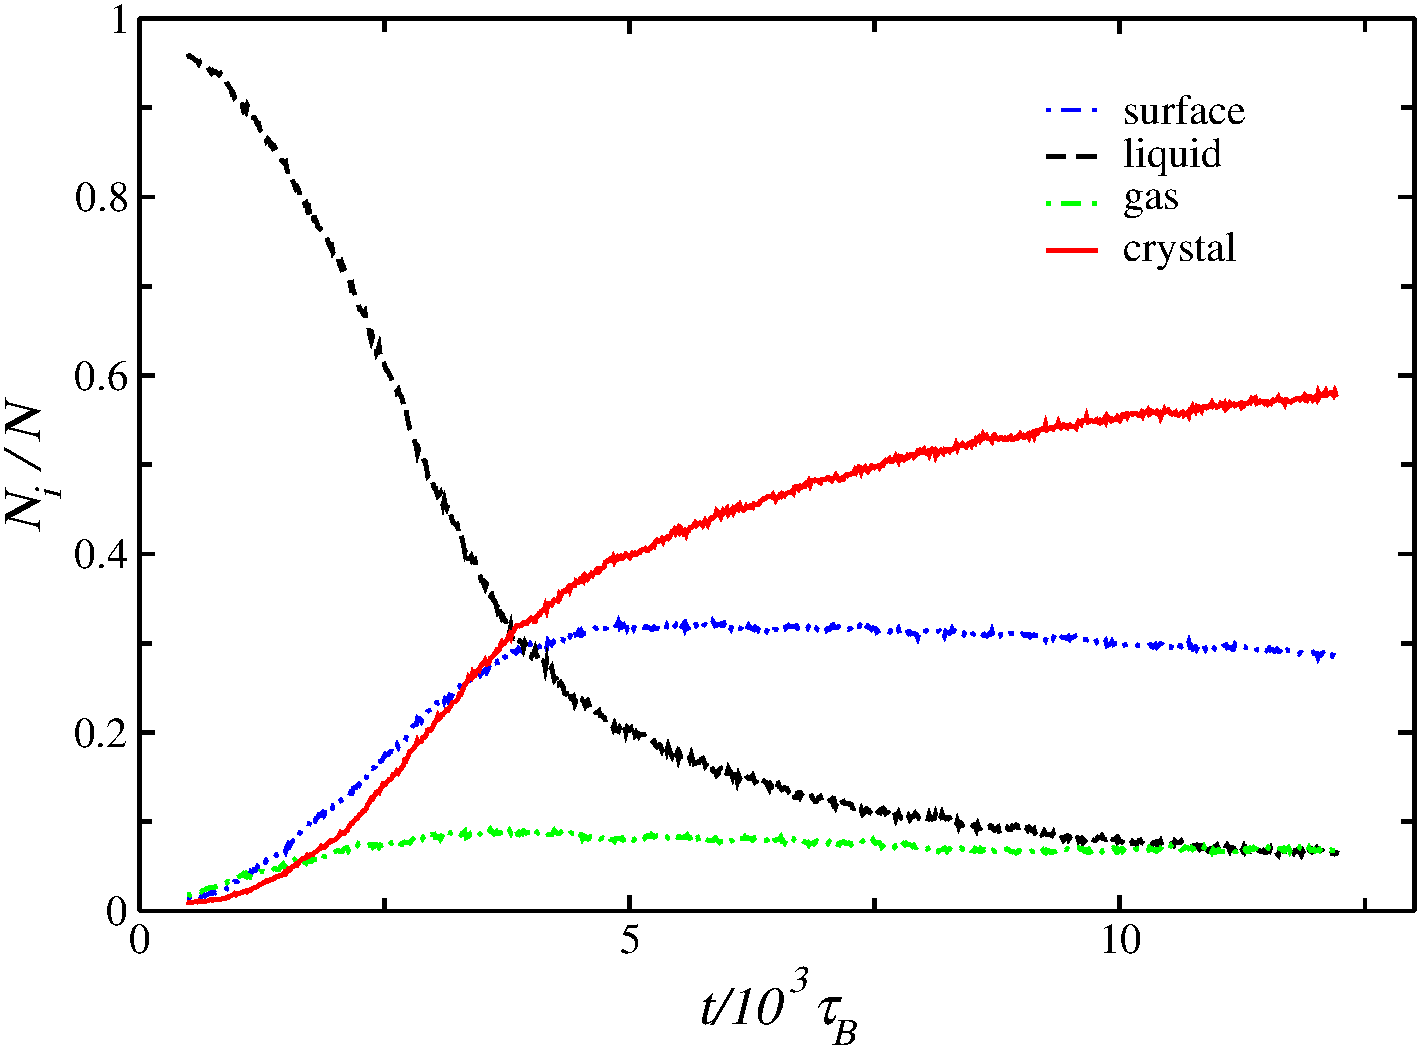
\includegraphics[width=10cm]{./fractions.pdf}
 % fractions.pdf: 681x503 pixel, 72dpi, 24.02x17.74 cm, bb=0 0 681 503
 \caption{{\bf Fraction of particles for each phase at $\phi\approx 0.30$ and $c_p=0.38$ mg/g}. The liquid
 fraction is depicted as a dashed black line, the gas fraction as a dotted-dashed green line, the surface
 fraction as a double-dotted-dashed blue line, while the crystal with a continuous red line.}
 \label{fig:fractions}
\end{figure}

Surface, gas and liquid particles are identified from the subset of non-crystalline particles depending
on their neighbouring particles. A particle with at least two neighbouring crystal particles is classified as
\emph{surface}. A particle that is neither solid nor surface, and has at least four neighbouring particles
is classified as \emph{liquid}. A particle which is neither solid, surface nor liquid is classified as \emph{gas}.
Figure~\ref{fig:fractions} plots the fraction of each state for the state point at $\phi\approx 0.30$ and $c_p=0.38$ mg/g

The distinction between gas and liquid phases is consistent with the analysis of volume fraction and composition
of the gas and liquid phases just after phase separation (and before crystallization). To analyse the fraction
of liquid and gas after phase separation we convert the position of particles into a continuous field smearing
the position of each particle with a Gaussian field of variance $5$ pixels, and then mapping the field
to a cubic grid with $10$ pixels spacing. In this way liquid and gas regions can be identified by
an appropriate threshold of the field.

\begin{figure}[!t]
 \centering
 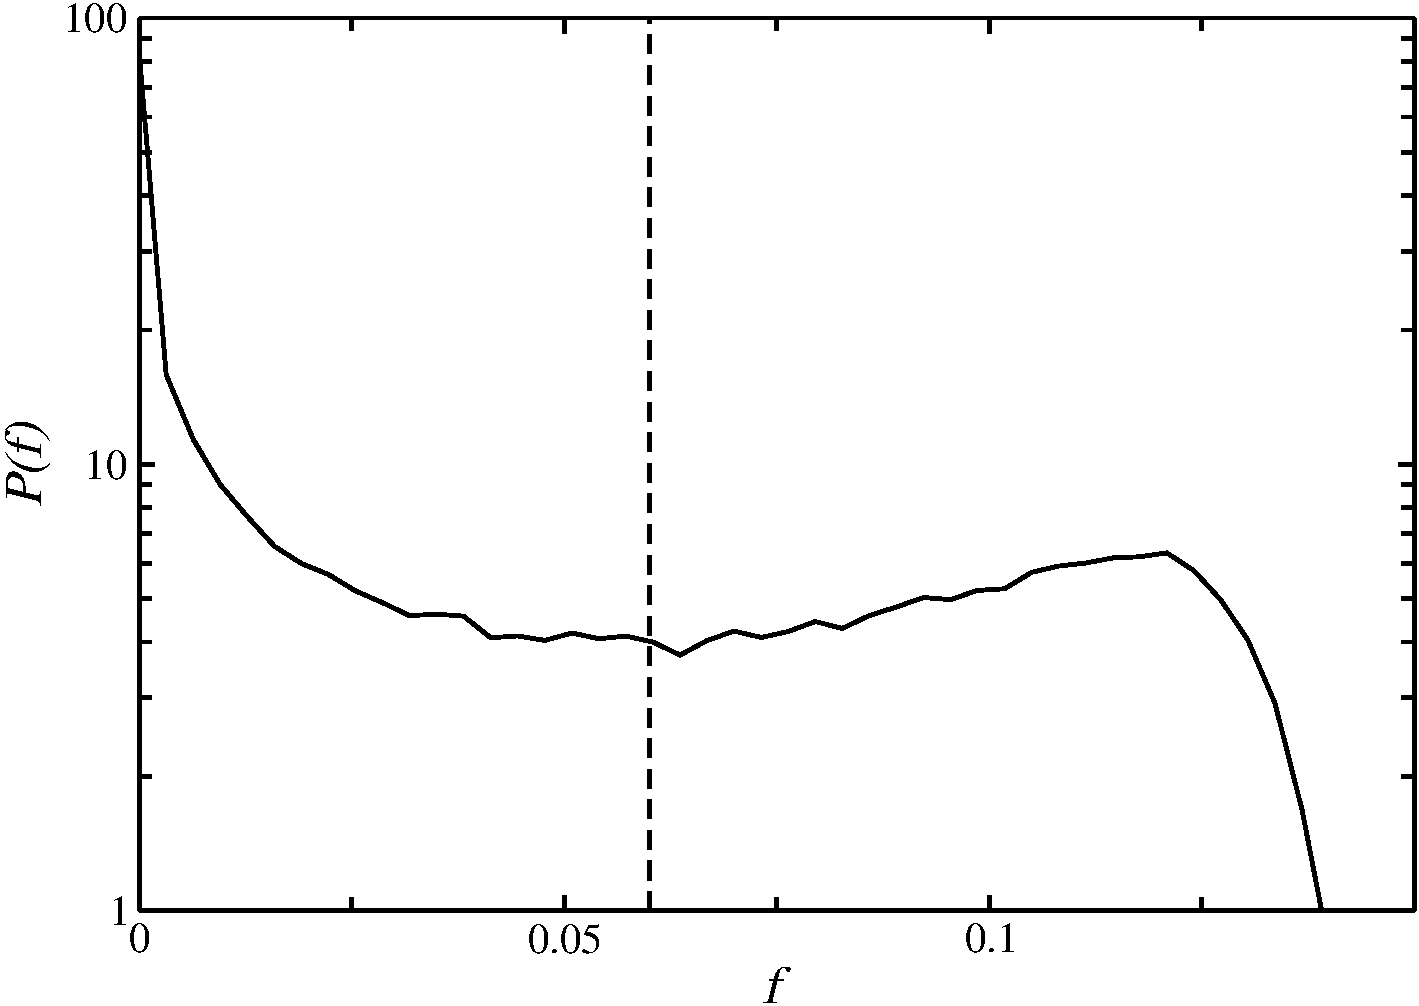
\includegraphics[width=10cm]{./field.pdf}
 % field.pdf: 681x483 pixel, 72dpi, 24.02x17.04 cm, bb=0 0 681 483
 \caption{{\bf Distribution function of the Gaussian field at $t=490\,\tau_{\rm B}$.} The Gaussian field is applied to
 a configuration just after phase separation and before crystallization. The vertical dashed line represents the
 field threshold $f=0.06$ used to distinguish between gas and liquid particles.}
 \label{fig:field}
\end{figure}

Figure~\ref{fig:field} shows the probability distribution of the field, where two peaks clearly indicate the presence
of gas/liquid coexistence. By choosing a threshold over the field of $f=0.06$ (vertical dashed line) we compute the fraction 
of particles in the solid and gas phases at $t=490\,\tau_{\rm B}$, just after phase separation. The results are consistent
with Fig.~\ref{fig:fractions}, where the number fraction of particles in the liquid state accounts for more than
$90\%$ of the particles just after phase separation.

\section*{Phase diagram}

The phase diagram is obtained in the framework of the generalized free volume theory. The colloids are considered as hard spheres and the polymers as an ideal gas. The centre of mass of a polymer cannot penetrate within $R$ of the surface of a colloid. Therefore the ideal gas is constrained to a free volume smaller than the total volume and that depends on the configuration (volume fraction) of the colloids and the polymer/colloid size ratio.

\subsection*{Adjusting theoretical and experimental phase diagrams}

\begin{figure}
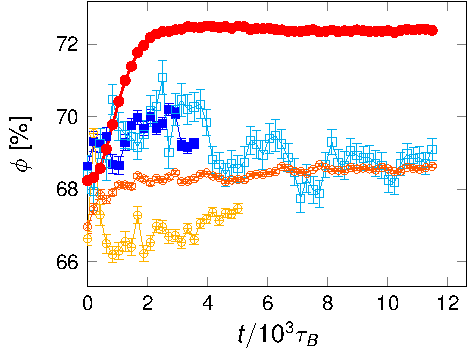
\includegraphics{local_phi12.pdf}%
\caption{{\bf Late stage of the evolution of the local volume fraction around colloidal particles having 12 nearest neighbours.} Samples are shown with the same colour code as in Fig.1 of the main text. In particular red circles correspond to the crystallizing sample at $\phi=0.33$ and $cp=0.38\,$mg/g.}%
\label{fig:local_phi12}%
\end{figure}

The volume fraction of a colloidal suspension is notoriously difficult to estimate experimentally~\cite{Poon2012}. It depends on the cube of the colloid diameter and is thus extremely sensitive to any error in size determination. Therefore here we determine the volume fraction directly from the phase behaviour and deduce a precise measure of the (effective) colloid diameter from it.

Our two constraints are (i) to have the final local volume fraction of the 12-neighboured particles in the crystallising sample to be equal to the theoretical equilibrium crystal volume fraction and (ii) to have the theoretical spinodal line to correspond to the gel region boundary. Starting from our initial estimates of $\sigma$ and $R$ we iteratively converge to $R=80$~nm, $\sigma = 2.25\,\mu$m and a crystal (without defects) at $0.723$.

\subsection*{Equation of state}

The free volume theory relies on an equation of state (EoS) for hard spheres to deduce phase boundaries of the colloids+polymers system. Canonically, the Carnahan-Starling (CS) EoS is used for the fluid and the equation of state by Hall for the crystal. CS is accurate for a wide range of volume fraction, but lacks a divergence below 1 although a divergence of the pressure is expected at the jamming point (random close packing $\phi_J\approx 0.64$). However CS is accurate up to 0.56. Therefore CS (coupled will Hall EoS) always describes accurately fluid-crystal coexistence since the fluid volume fraction is at most 0.495.

The gas spinodal line is given by an inflexion point of the free energy, a local property of the equation of state. Therefore, the locally correct CS EoS is able to describe accurately the gas side of the spinodal region up to 0.56. The iterative process described above can be done only using CS EoS.

However, the liquid side of the binodal and spinodal lines obtained from CS EoS reach unphysically high volume fractions (above close packing), making comparisons with the measured liquid compositions impossible.

Indeed our small polymer/colloid size ratio pushes the gas-liquid critical point to high volume fractions, exemplifying the failure of CS EoS. Adding a divergence at Jamming into CS equation of state is not trivial. Attempts by Lefebre~\cite{LeFevre1972} and Kolafa~\cite{Kolafa2004} match CS at low density, have the right divergence close to jamming but far less than CS at intermediate volume fractions (0.5-0.56), the exact range where our critical point lies. Here we decided to use an equation by Liu~\cite{Liu2006a} that is completely equivalent to CS up to 0.56 and then show good agreement with simulation data near jamming.
%
The Liu EoS allows us to draw a phase diagram that is in qualitative agreement with the measured liquid compositions.

\section*{Transition probabilities}
\begin{figure}
 \centering
 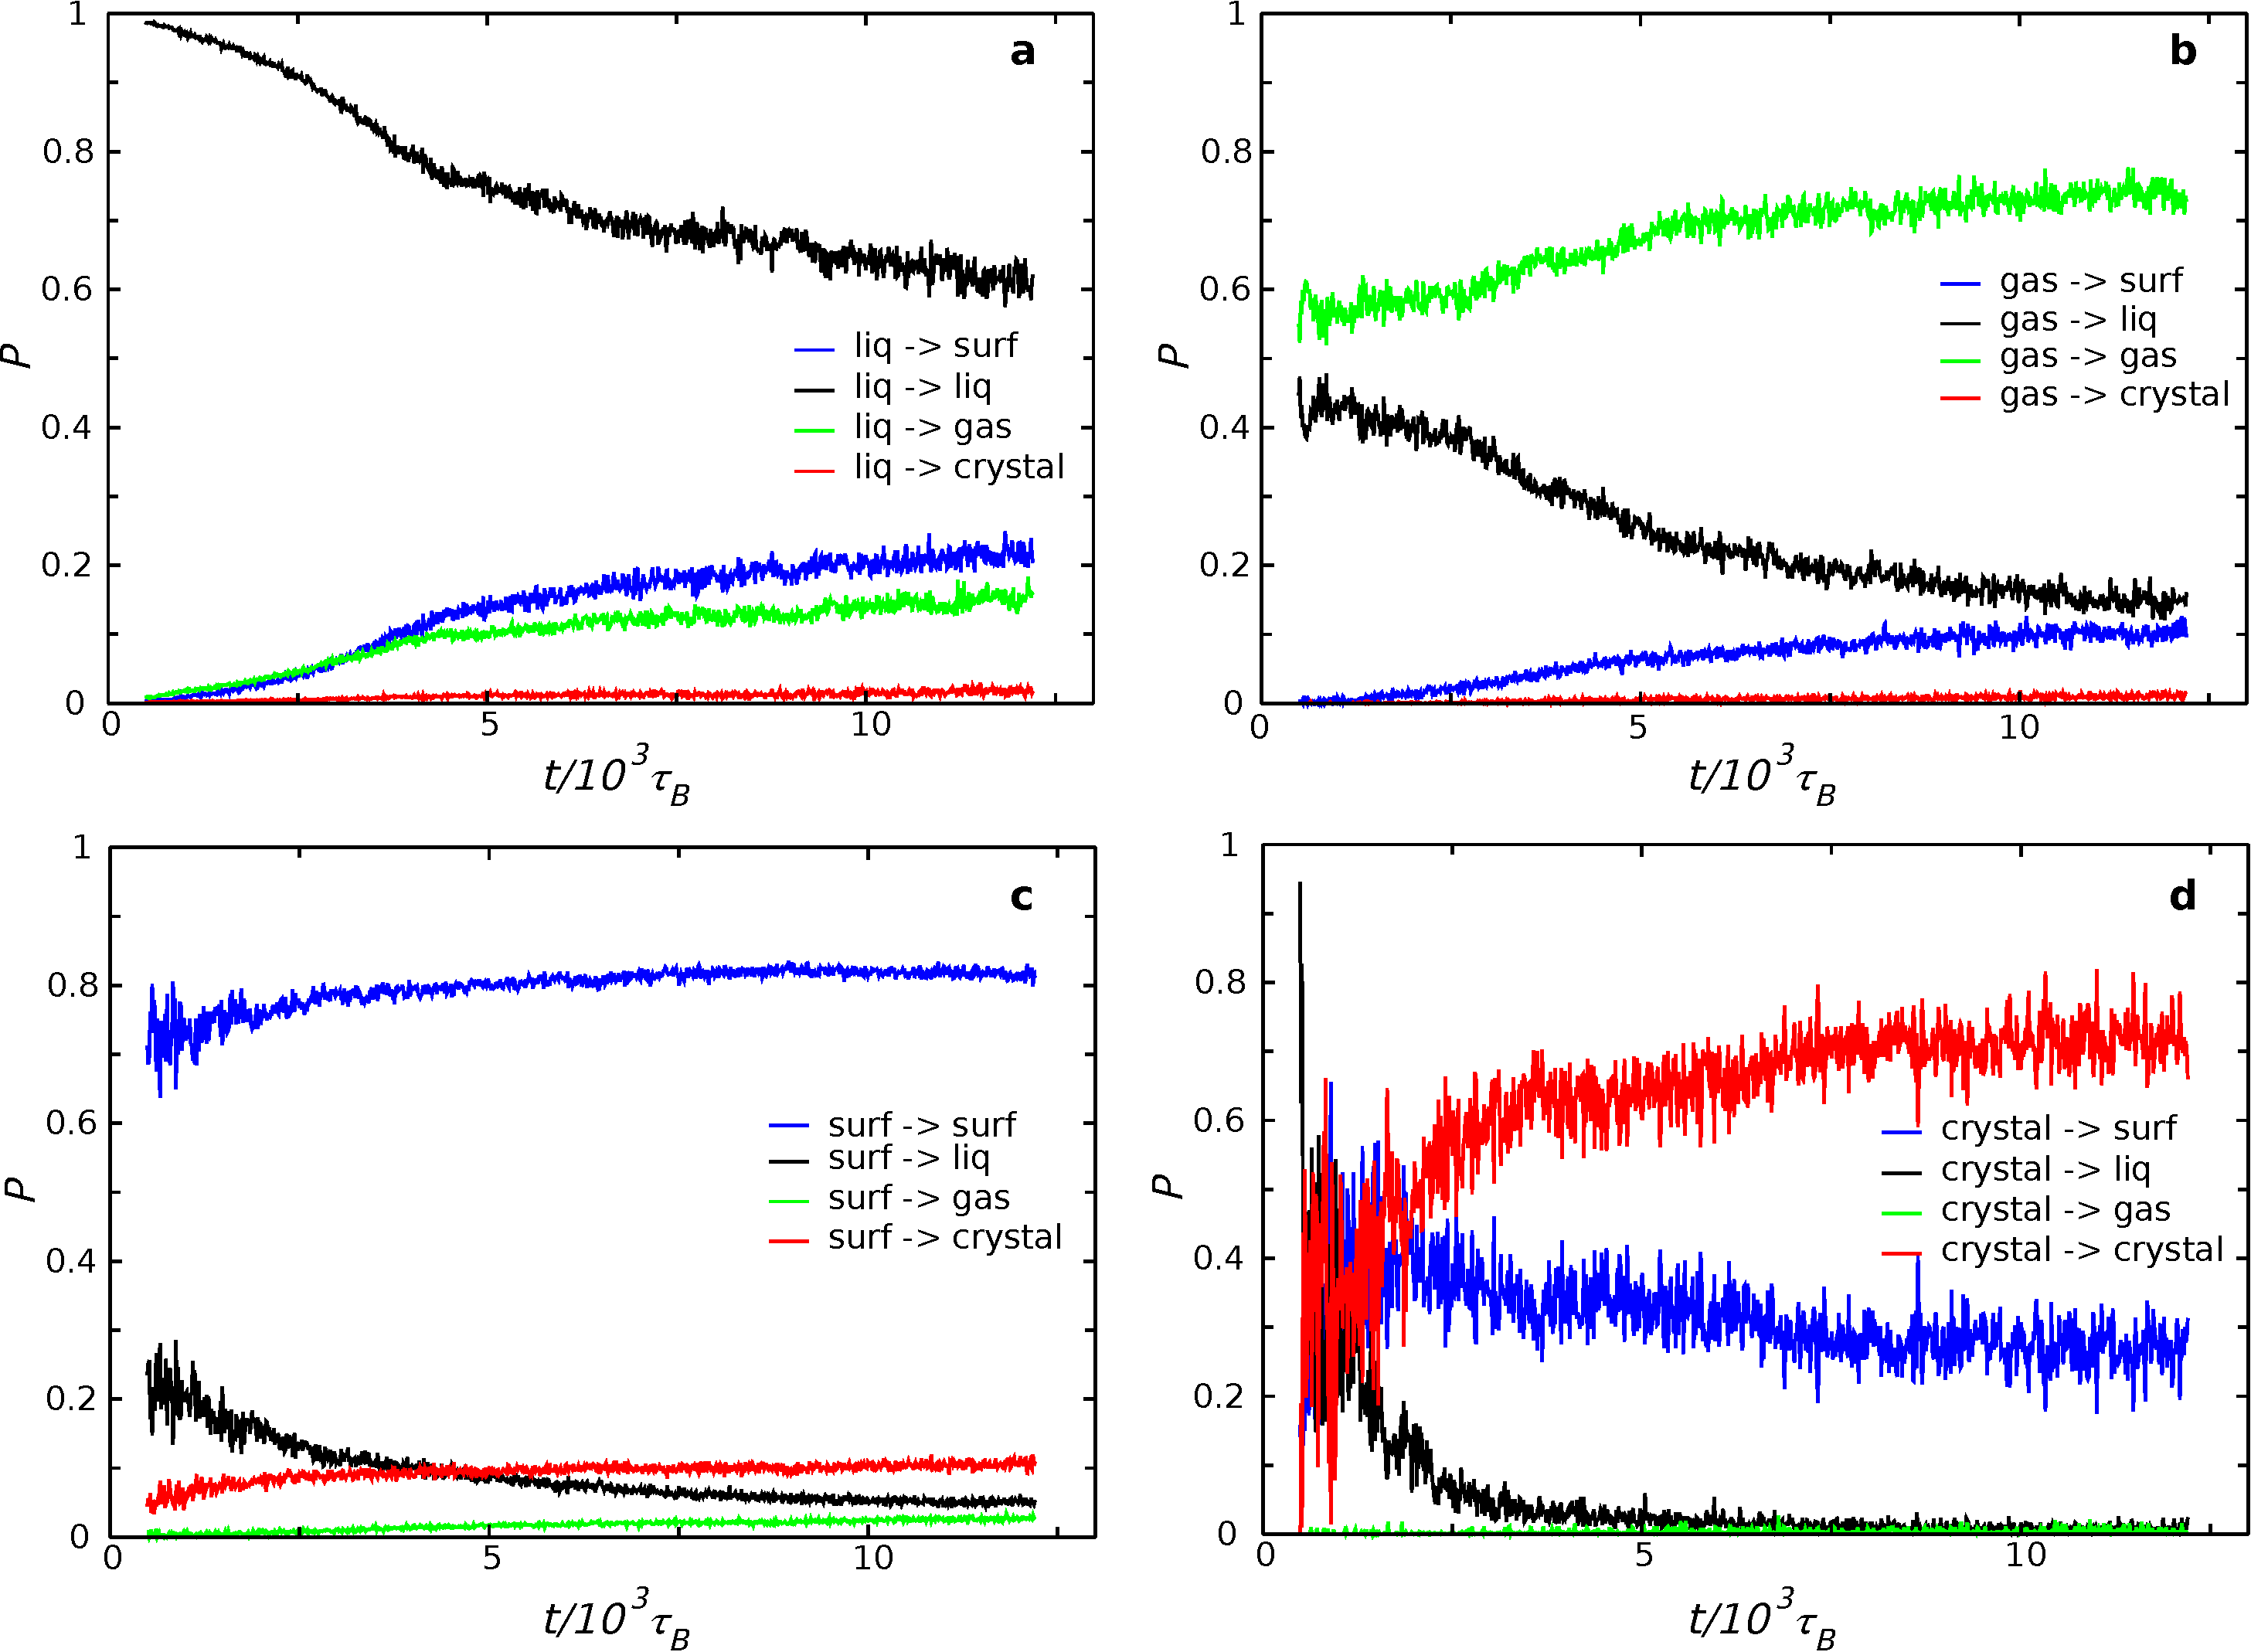
\includegraphics[width=14cm]{./sfig1.pdf}
 % sfig1.pdf: 1398x1026 pixel, 72dpi, 49.32x36.19 cm, bb=0 0 1398 1026
 \caption{{\bf Transition probabilities during the formation of the crystal-gel.}
 {\bf a,} Transition probabilities from the liquid state;
 {\bf b,} Transition probabilities from the gas state;
 {\bf c,} Transition probabilities from the surface state;
 {\bf d,} Transition probabilities from the crystal state. In all panels the possible
 transition states are surface (blue), liquid (black), gas (green) and crystal (red).
 See the text for the definition of each state.
 }
 \label{fig:probabilities}
\end{figure}

In Fig.~\ref{fig:probabilities} we plot the transition probabilities between the gas, liquid, crystal
and surface states, as defined in the previous Section. Each panel represents the transition probability
of a different state: {\bf a} for the liquid state, {\bf b} for the gas state, {\bf c} for the surface state,
and {\bf d} for the crystal state. The results indicate that the liquid phase preferentially transforms into
the surface state (as a precursor to crystallization), which accounts for the \emph{direct crystallization channel}
that was described in the main text. A high percentage of liquid transforms also in the gas phase. The gas phase itself
transforms back into liquid or into surface particles, a process which
is linked to the \emph{Bergeron process}. These results support the idea that both channels are active
crystallization pathways. Direct transformation of either liquid or gas into crystalline states is almost absent,
indicating that our surface state indeed captures the precursor particles that attach to nuclei and later crystallize.
Surface particles in fact, first transform preferentially into the liquid state, but at later time instead transform
more prominently into the crystal state. The transformation of crystals into the surface state, represents the first
step of the \emph{Ostwald process}, but this channel is limited by the small rate of conversion of surface particles
into the gas state.

\section*{Capillary experiment}

\begin{figure*}[!t]
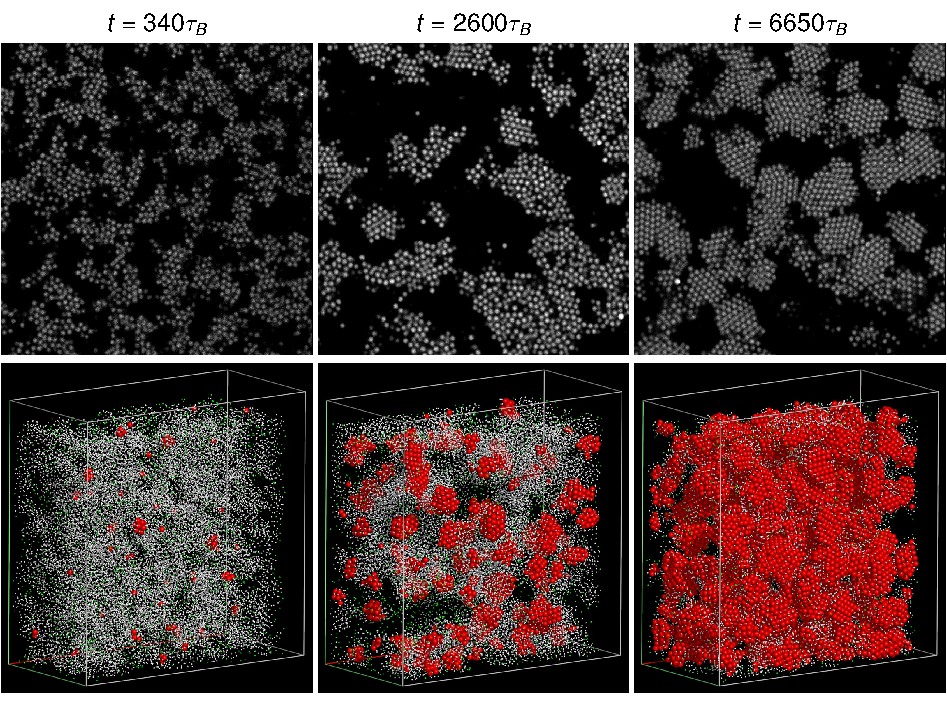
\includegraphics{capillary.pdf}
\caption{\textbf{Capillary experiment reproducing the crystal-gel state.} The colloid volume fraction is $\approx 0.33$ and the polymer concentration is $0.40\,$mg/g. Top row: Confocal slices showing the initial network, crystallising network and final crystal-gel network. Bottom row: Reconstructions from confocal coordinates. Particles are drawn to scale and coloured according to their phase. Red: crystal; white: liquid; green: gas; surface: blue. To highlight the crystalline regions, liquid, gas, surface particles are drawn to a tenth of the crystalline particle size.}
\label{fig:capillary}
\end{figure*}


The use of a reservoir of a salt solution through a semi-permeable membrane, allowed us to follow the entire microscopic dynamics in absence of spurious flows, from the first stages of phase separation to the formation of the crystal-gel state. In order to confirm the reproducibility of the crystal-gel state, we conducted experiments in a more traditional capillary setting, where all components of the suspension are pre-mixed in a sealed cell. A typical example is
shown in Fig.~\ref{fig:capillary}, where a system with the colloid volume fraction of $\approx 0.33$ and the polymer concentration of $0.40\,$mg/g is considered.
The figure shows the time evolution of the sample at three different times, just after phase separation ($t=340\,\tau_{\rm B}$), and during
crystal-gel formation ($t=2600\,\tau_{\rm B}$ and $t=6650\,\tau_{\rm B}$). The top-row shows images from quasi two-dimensional confocal slices, while the bottom-row shows
the three-dimensional reconstruction after single-particle tracking, where crystalline particles are highlighted in both size (large) and color (red), surface particles
are depicted in blue, gas in green and liquid in white.

\bibliographystyle{naturemag2}
\bibliography{biblio}

\clearpage

\section*{Supplementary Movie 1}
This movie shows the early stage of gelation process of $\phi\approx 0.30$ and $c_p=0.38$ mg/g, from the original confocal images at the same z-position as Fig.~3a. Total duration is 1160 s (530~$\tau$). We quickly started scanning the sample after exchanging the salt-reservoir with the solvent including salt. At the beginning, salt had not reached the scanning volume and colloids were dispersed by electrostatic repulsion. At 0:02 in the movie, salt diffused into the scanning volume and screened the surface charges of colloids. Then, colloids immediately initiated phase separation by short-ranged attractions.

\section*{Supplementary Movie 2}
This movie shows the late stage after Supplemental Movie 1 with scanning duration of 27000~s (12300~$\tau$). 
Please note that there is a large difference in the frame rate between Movie 1 and 2. 

\section*{Supplementary Movie 3}
Same as Supplementary Movie 2, but with computer rendered trajectories obtained from the tracking of the colloidal particles.
Particles are colored according to the following code: crystal (red), surface (blue), gas (green) and liquid (white).
For display purposes, crystalline particles and gas particles are respectively 400\% and 50\% bigger than other particles (liquid or surface).


\end{document}
